%%This is a very basic article template.
%%There is just one section and two subsections.



\documentclass{report}


\usepackage{microtype}
\usepackage[tight,footnotesize]{subfigure}
\usepackage[T1]{fontenc}
\usepackage[latin1]{inputenc} % Input in ISO 8859-1 (Latin1)

\usepackage{ae}               % Almost european, virtual T1-Font
\usepackage[pdftex]{graphicx}
\usepackage{vmargin}          % Adjust margins in a simple way
\usepackage{fancyhdr}         % Define simple headings
\usepackage{subfigure}
\usepackage{url}
\usepackage[absolute,overlay]{textpos}
\usepackage{tikz}
\usepackage[english]{babel}
\usepackage{algorithm}		  % Code-Listings
\usepackage{algorithmic}	  % Code-Listings
\usepackage{hyperref}
\usepackage{listings}
\usepackage{dirtree}
\usepackage{multirow}
\usepackage{booktabs}
\usepackage{wrapfig}
\newcommand{\DS}{DynamicSpotter }
\newcommand{\hlight}[1]{\textcolor[rgb]{0.8,0,0.2}{#1}} 
\newcommand{\link}[1]{\textcolor[rgb]{0.0,0.0,1.0}{\href{#1}{#1}}}
\definecolor{mygreen}{rgb}{0,0.6,0}
\definecolor{mymauve}{rgb}{0.58,0,0.82}
\renewcommand*\thesection{\arabic{section}}
\selectlanguage{english}
\begin{document}


\begin{titlepage}
\begin{center}
\textsc{}\\[5cm]
% Oberer Teil der Titelseite:
\begin{textblock*}{115mm}(65mm,70mm)
\centering{

\includegraphics[scale=0.3]{figures/spotter_logo.pdf}
}
\end{textblock*}

\textsc{\LARGE A Framework for Automatic Diagnosis}\\[0.3cm]
\textsc{\LARGE of Performance Problems}\\[1.0cm]
\textsc{---}\\[1.0cm]
\textsc{\Large User Guide}\\[3.0cm]
% Title
\newcommand{\HRule}{\rule{\linewidth}{0.5mm}}

\begin{minipage}{0.48\textwidth}
\centering
\Large{
\textbf{Alexander Wert}}
\large{
\\alexander.wert@kit.edu\\ Am
Fasanengarten 5\\
Software Design and Quality
\\
Karlsruhe Institute of Technology
}
\end{minipage}
\hfill
\begin{minipage}{0.48\textwidth}
\centering
\Large{
\textbf{Denis Kn\"opfle}}\\
\large{
denis.knoepfle@sap.com\\
Vincenz-Prie{\ss}nitz-Stra{\ss}e 1\\
SAP AG\\
\textcolor[rgb]{1,1,1}{ }}
\end{minipage}
\\[3.0cm]

\Large{\textbf{Contributors}}\\
\Large{Alexander Wert},
\Large{Christoph Heger},
\Large{Roozbeh Farahbod},
\Large{Denis Kn\"opfle},
\Large{Peter Merkert},
\Large{Marius Oehler},
\Large{Henning Schulz}
\vfill
\HRule

\begin{minipage}{0.4\textwidth}
\begin{flushleft} 
\large \link{http://sopeco.github.io/DynamicSpotter}
\end{flushleft}
\end{minipage}
\hfill
\begin{minipage}{0.4\textwidth}
\begin{flushright} 
\large \today
\end{flushright}
\end{minipage}


% Unterer Teil der Seite


\end{center}

\end{titlepage}



% \begin{textblock*}{115mm}(57mm,70mm)
% \centering{
% 
\includegraphics[scale=0.35]{figures/spotter_logo.pdf}
% }
% \end{textblock*}
% 
% \title{\textsc{\LARGE A Framework for Automatic Diagnosis of Performance Problems}\\---\\User
% Guide\vspace{100px}}
% 
% \author{\textbf{Alexander Wert}\\alexander.wert@kit.edu\\ Am
% Fasanengarten 5\\
% Software Design and Quality
% \\
% Karlsruhe Institute of Technology}
% 
% \maketitle
\tableofcontents
\newpage


\section{The Approach behind \DS}
\label{sec:approach}
\DS is a framework for automatic detection of performance problems in Java-based enterprise software systems. Therefore,
\DS combines the concepts of software performance anti-patterns with systematic experimentation. 

Software performance
anti-patterns (SPAs) \cite{smith2000software,smith2002software,smith2003more,smith2003new} describe common, recurring
design or implementation mistakes leading to impaired software performance. As a big portion of software performance
problems exhibit recurring nature, the concept of SPAs is a means to identify such problems in different
contexts (different target-systems, environments, etc.) by searching for the generic patterns, or characteristics,
different SPAs exhibit. 

If the system under test (SUT) is implemented and can be executed, performance tests allow to
gain insights on its performance behaviour. There are three important things to know about performance tests: 
\begin{enumerate}
  \item Usually, a load driver (such as JMeter\texttrademark \cite{jmeter} or HP LoadRunner \cite{loadrunner}) is used to
generate a set of virtual users processing a script, which describes the work of single users. 
  \item  During
load generation, performance metrics are retrieved from the SUT using instrumentation and monitoring techniques. 
  \item The gathered measurement data is analyzed to provide insights on particular performance engineering tasks.
\end{enumerate}
In our context, the gathered measurement data can be mapped to the
generic characteristics defined by individual SPAs. If measurement data matches certain pattern of an SPA, there is a
high chance that the SUT contains the corresponding anti-pattern. 
However, the following circumstances render the detection of different SPAs with a single performance test impractical.
Different SPAs refer to different parts, performance metrics and granularity levels of the SUT. Thus, in order
to investigate different SPAs in a SUT as part of a single performance test, detailed and excessive instrumentation of
the SUT is required.
However, as each instrumentation instruction comes with a performance overhead, excessive instrumentation yields a
high overhead which distorts measurement data, rendering analysis on this data useless. Hence, an experiment-based
process is needed in which individual SPAs are investigated as part of individual performance tests (in the following
called \emph{experiments}). In this way, during each experiment the SUT is instrumented selectively for the
corresponding SPA, providing detailed measurement data while keeping the performance overhead of the instrumentation
low. 

Though, the experiment-based process significantly mitigates the problem of the performance overhead introduced by the
instrumentation, it increases the manual effort required to configure, execute and analyze each single experiment
referring to an SPA. Moreover, the larger the set of investigated SPAs the more experiments are required, and with that
the time required to execute the experiments grows. However, this problem can be mitigated by using an appropriate
structure of the SPAs. Though there is a large set of different recurring performance problems, many of those problems
share common characteristics and symptoms. Hence, performance problems can be structured in a systematic way, yielding a
hierarchy from high level symptoms to specific root causes of the problems. 
An example of such a hierarchy is depicted in Figure~\ref{fig:hierarchy}.

\emph{Varying Response Times} is a symptom. \emph{The Ramp}~\cite{smith2003new} and \emph{Traffic
Jam}~\cite{smith2002software} are potential causes of \emph{Varying Response
Times}.
\emph{The Ramp} occurs if response times of an application increase during
operation. Such a behaviour can, for example, occur if the
application contains \emph{Dormant References}~\cite{rayside2007object}, i.e.,
the memory consumption of the application is growing over time. The root cause
is \emph{Specific Data Structure}s which are growing during operation or which are not properly
disposed.
The \emph{Traffic Jam} performance antipattern constitutes another cause of \emph{Varying Response Times}. 
A \emph{Traffic Jam} occurs if many concurrent threads or processes are waiting for the same passive resource ((like
semaphores or mutexes)) or active resource (like
CPU or hard disk). In the first case, we have a typical \emph{One Lane Bridge}~\cite{smith2000software}
whose critical resource needs to be identified. We focus on \emph{Synchronization Points}, \emph{Database Locks}, and \emph{Pools} as potential root causes.
In the case of limited physical resources, the root cause can only be a specific \emph{Bottleneck Resource}.
Further examples on a performance problem hierarchy can be found in \cite{wert2013supporting, wert2014automatic,
wert2013performance}. 

A hierarchy as depicted in Figure~\ref{fig:hierarchy} can be utilized as a search
tree, in order to systematically search for performance problems by conducting a depth-first search on the tree. In
particular, a branch or sub-tree of the hierarchy does not need to be investigated if the problem corresponding to the
sub-tree's root node is not present in the SUT. In our example, possible root causes for \emph{The Ramp} do not need to
be investigated if \emph{The Ramp} itself has not been detected in the SUT. In this way, many unnecessary experiments
can be avoided, saving experimentation time and effort. 

\begin{figure}[t]
\subfigure[An exemplary hierarchy of performance problems (from \cite{wert2013supporting}) \label{fig:hierarchy}]{
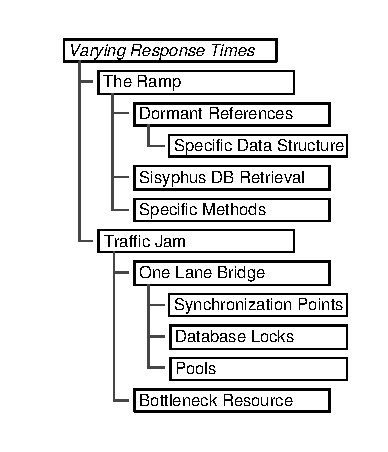
\includegraphics[width=0.3\textwidth]{figures/hierarchy.pdf}
}
\hfill
\subfigure[Overview on the \DS approach (graphic from \cite{wert2014automatic}) \label{fig:spotter}]{
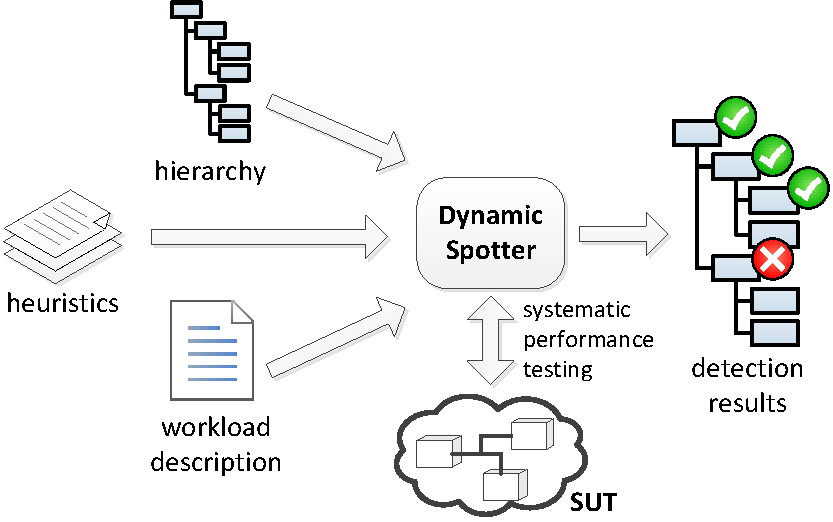
\includegraphics[width=0.6\textwidth]{figures/spotter.pdf}
}
\caption{\DS approach}
\end{figure}

\DS utilizes the concept of hierarchically structuring performance problems (respectively SPAs) in order to automate
the search for recurring performance problems (SPAs) by systematically executing measurement experiments. The high level
approach behind \DS is depicted in Figure~\ref{fig:spotter}. \DS takes a performance problem hierarchy (as described
before) as input. For each node of that hierarchy, performance experts define a heuristic responsible to decide on the
existence of the corresponding problem. To this end, a heuristic executes a series of experiments, observes certain
performance metrics and analyzes them to make a decision. (Note: Both, the hierarchy and the corresponding heuristics
are generic artifacts which do not depend on the SUT under test and, thus, can be reused in other contexts.) For
instance, in order to detect a \emph{One Lane Bridge}, the corresponding heuristic may execute a set of experiments with
different load intensities, while observing end-to-end response times. If response times significantly increase with
the load, while none of the hardware resources is utilized to capacity, the SUT contains an OLB.
For execution of experiments, a load script (\emph{workload description}) specifies the work of single virtual users. 
Traversing the hierarchy and applying corresponding heuristics for each performance problem of the hierarchy, \DS
generates a detection result report. The report states for each node in the hierarchy whether the corresponding
problem exists in the SUT and, where appropriate, points to the root cause and location in the SUT of a detected
problem.



\section{Architecture of \DS}
\label{sec:architecture}

\begin{figure}[p]
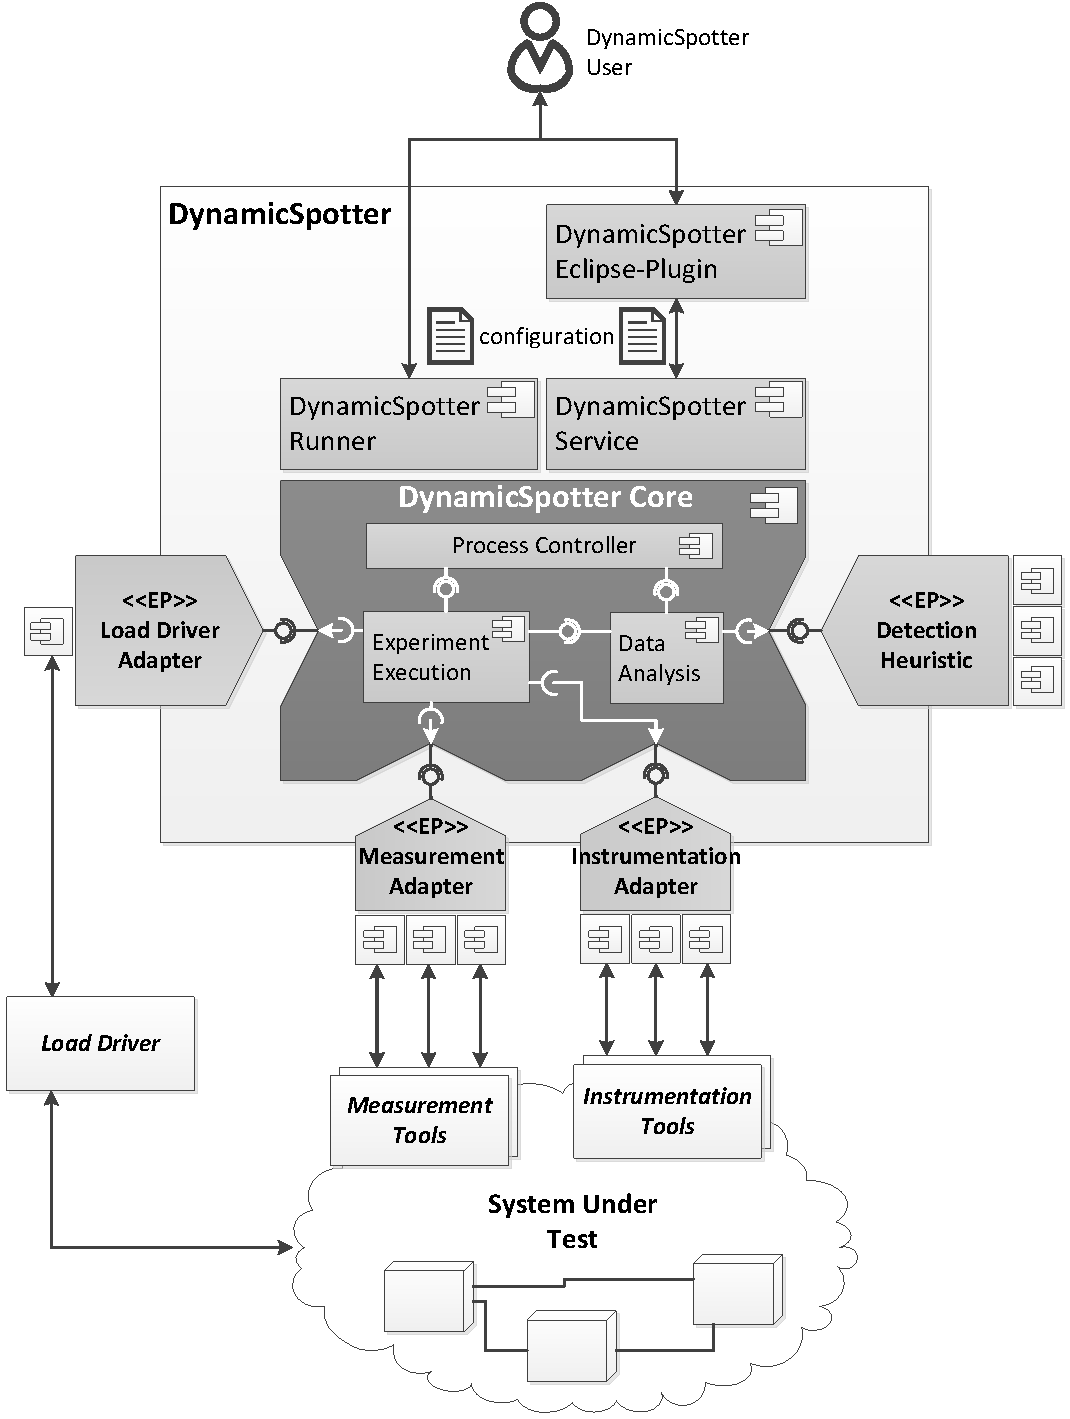
\includegraphics[width=\textwidth]{figures/architecture.pdf}
\caption{\DS architecture}
\label{fig:architecture}
\end{figure}
As described in Section~\ref{sec:approach}, \DS is a framework for automatic detection of performance problems. The
architecture of \DS is depicted in Figure~\ref{fig:architecture}. The main component of \DS (\texttt{\DS Core}) realizes
the logic for automating performance tests and data analysis. In particular, \texttt{\DS Core} is responsible for
coordinating  the instrumentation of the system under test (SUT), the monitoring process, gathering and
pre-processing measurement data, as well as analyzing data. Furthermore, \texttt{\DS Core} implements the high level
process of iterating a performance problem hierarchy (cf. Component \texttt{Process Controller} in
Figure~\ref{fig:architecture}), as described in Section~\ref{sec:approach}.
The \texttt{Experiment Execution} component is responsible for automating experiment execution, while the \texttt{Data
Analysis} component conducts the data analysis task for individual performance problems according to the detection rules
defined for corresponding performance problems in form of \emph{Heuristics}.
For each sub-task, \DS provides extension points (denoted with \texttt{\(\ll\)EP\(\gg\)} in Figure~\ref{fig:architecture})
allowing to provide adapters for specific implementations or tools used for instrumentation, monitoring, workload
generation, and data analysis:

\begin{itemize}
  \item \textbf{\(\ll\)EP\(\gg\) Load Driver Adapter:} The \texttt{Load Driver Adapter}
  extension point provides means to use existing load driver tools like JMeter, Faban or HP LoadRunner for workload generation.
  In particular, a \texttt{Load Driver Adapter} needs to provide means to control the execution of performance tests
  programmatically. Furthermore, the adapter realizes a remote communication between \DS and the remotely running load
  generation tool.
  \item \textbf{\(\ll\)EP\(\gg\) Instrumentation Adapter:} The \texttt{Instrumentation Adapter} extension point allows
  to provide adapters for instrumentation tools like DiSL, Kieker, our own instrumentation tool AIM (Adaptable Instrumentation and
Monitoring), etc. Thereby, \DS uses a generic instrumentation description model (IDM) to decouple the instrumentation
description from the tool realizing it. Thus, an instrumentation adapter for a specific instrumentation tool has to
realize the transformation from the IDM instances to the tool-specific representation of the instrumentation
description.
  \item \textbf{\(\ll\)EP\(\gg\) Measurement Adapter:} While an instrumentation adapter is solely responsible for
  instrumenting the SUT, a \texttt{Measurement Adapter} is used to enable and disable data collection, as well as to
  transform and transfer data from the monitoring tool to \DS in a common data representation format. Though a
  specific instrumentation adapter and a measurement adapter are often realized within one external tool, they represent
  conceptually different tasks. In such a case, adapters for both extensions points are required, even if only one tool
  realizes both tasks. 
  \item \textbf{\(\ll\)EP\(\gg\) Detection Heuristic:} As described in Section~\ref{sec:approach}, \DS uses a
  performance problem hierarchy and corresponding heuristics to guide the detection process. Both artifacts need to be
  provided by performance experts. For each performance problem defined in the hierarchy, a performance expert can
  provide a \texttt{Detection Heuristic} extension which is then responsible to define the experiments and analyse the
  corresponding measurement data for the corresponding performance problem. 
\end{itemize}

Depending on the size of the SUT, \DS may use several \texttt{Instrumentation Adapters}, \texttt{Measurement Adapters}
and \texttt{Load Driver Adapters}. A set of adapters to be used in a specific application context of \DS determines the
\emph{Measurement Environment} for \DS. In order to use \DS, a user has to specify the \emph{Measurement Environment} in
a \texttt{configuration}. Thereby, a user either can start a headless \DS process (cf. \DS Runner in Figure~\ref{fig:architecture})
providing the \texttt{configuration} as input, or, the user harnesses the \texttt{\DS Eclipse-Plugin} to build a \texttt{\DS configuration} in an interactive
way, trigger the automatic detection process, and finally, examine the detection results in the graphical user
interface. The \texttt{\DS Eclipse-Plugin} communicates with a \texttt{\DS Service} layer running on top of
the \texttt{\DS Core}. Utilizing the description of the \emph{Measurement Environment}, \DS identifies required
extensions and establishes connections to the corresponding external instrumentation, measurement and load generation
tools. \DS is then able to automatically run performance tests and analyze measurement data as defined in the heuristics
of the individual performance problems from the performance problem hierarchy. As a result, \DS provides a report to the
user stating which performance problems have been detected.  

\section{DynamicSpotter - Getting Started}
In this section, we demonstrate the usage of \DS on a very simple scenario. Some of the \DS plugins we use in this
scenario are just simple examples (e.g. the plugin for load generation) to demonstrate the \DS framework. In real
scenarios more sophisticated \DS plugins would be used, such as the JMeter plugin for load generation.

We show how to configure the target application, set-up \DS, run \DS diagnosis and view diagnosis
results.


\subsection{Requirements}
In order to run through the demo example in this section, the following is required:
\begin{itemize}
  \item JDK (tested with JDK 1.7)
  \\ \link{http://www.oracle.com/technetwork/java/javase/downloads/jdk7-downloads-1880260.html}
  \item An Eclipse standard installation (tested with Eclipse Kepler) 
  \\ \link{http://www.eclipse.org/downloads/packages/eclipse-standard-432/keplersr2}
\end{itemize}

\subsection{All-In-One Demo Example}
All binaries required for executing the demo scenario are available in the \texttt{All-In-One} archive which you can
download from the following URLs:
\newline
\newline
Windows: \link{http://i43vm-saas.ipd.uka.de:8082/artifacts/demo-all-in-one.zip}
\newline
Linux: \link{http://i43vm-saas.ipd.uka.de:8082/artifacts/demo-all-in-one.tar.gz}
\newline
\newline
Unpack the archive in any directory. The content of the archive is the following:
\dirtree{%
 .1 /.
 .2 demo-app.jar.
 .2 instrumentation-agent.jar.
 .2 ds-server.jar.
 .2 plugins.
 .3 instrumentation-plugin.jar.
 .3 measurement-plugin.jar.
 .3 loadgeneration-plugin.jar.
 .3 detection-olb-plugin.jar.
 .3 detection-ramp-plugin.jar.
 .2 ds-eclipse-ui.jar.
 .2 loadScript.
 .3 org.
 .4 spotter.
 .5 ext.
 .6 demo.
 .7 load.
 .8 VUser.class.
 .2 ds-cl-runner.jar.
 .2 demo-config.
 .3 hierarchy.xml.
 .3 mEnv.xml.
 .3 spotter.conf.
}
The \texttt{demo-app.jar} comprises the target demo application used in the following scenario as the system under test
(SUT). In order to be able to retrieve some performance data from the target application, we provide an
\texttt{instrumentation-agent.jar} which allows to instrument the target application and gather measurement data.
Thereby, \texttt{instrumentation-agent.jar} contains the Java-agent from our own instrumentation tool AIM
(adaptable instrumentation and monitoring) also available on GitHub (cf. Section~\ref{sec:links}). The
instrumentation agent needs to be started with the target application as an additional JVM parameter, which we will
explain later in more detail. The \DS framework is bundled in the \texttt{ds-server.jar}. The \texttt{plugins} directory
contains a set of extensions for \DS which we need for this demo scenario. In particular (according to the architecture
described in Section~\ref{fig:architecture}), we need an instrumentation (\texttt{instrumentation-plugin.jar}) and
measurement adapter (\texttt{measurement-plugin.jar}) to connect to the instrumentation agent, a load generation
plugin (\texttt{loadgeneration-plugin.jar}) to be able to submit load on the target application, and some detection
heuristics (\texttt{detection-olb-plugin.jar} and \texttt{detection-ramp-plugin.jar} ) for the analysis of certain
performance problems. For simplicity, in this scenario we use only two detection heuristics, one for detecting a One
Lane Bridge anti-pattern (software bottleneck) and a heuristic for the detection of the Ramp anti-pattern (slowly
decreasing software performance). The \texttt{ds-eclipse-ui.jar} is a plugin for Eclipse comprising the graphical user
interface for \DS. Finally, the \texttt{loadScript} directory contains a load scenario for the target application in
form of a Java class (including the package-directory structure). In order to run \DS in a batch mode from the command
line one can use the \texttt{ds-cl-runner.jar}. The demo-config folder contains demo configuration for the execution of
\DS from command line.

\subsection{Demo Application}
\label{sec:demoApp}
For our demonstration scenario we use a dummy application providing two services. A service containing a One Lane Bridge
(OLB) performance anti-pattern and a second service without any performance problems. Listing~\ref{lst:demoApp} shows
the code of the target dummy application. The \texttt{DummyApp} class comes with two REST services: \texttt{testOLB} and
\texttt{fibonacci}. The first service contains an OLB anti-pattern manifested in a call to a synchronized method
(\texttt{OLB.olbMethod()}) becoming a software bottleneck. This dummy application runs on a Web server such that users
of that application can access the services via a REST interface.

\lstinputlisting[language=Java, frame=single,
caption=Code of the Demo
Application,commentstyle=\color{mygreen},keywordstyle=\color{blue},stringstyle=\color{mymauve},tabsize=3, label=lst:demoApp]{code/DemoApp.txt}

In order to execute the demo application execute the following command in the directory you have unpacked the all-in-one
archive to:
\begin{lstlisting}[language=sh,morekeywords={java,javaagent,\-jar}, frame=single]
java -javaagent:instrumentation-agent.jar -jar demo-app.jar start
\end{lstlisting}
With \texttt{-jar demo-app.jar start} we instruct the demo application to start. Additionally we provide a
\texttt{-javaagent} JVM argument pointing to the \texttt{instrumentation-agent.jar}. This Java agent is later used to
dynamically instrument the bytecode of the target application in order to retrieve different types of measurement data.
The Java agent starts a REST service on port \texttt{8888}.

\subsection{Load Script}
\label{sec:loadScript}
As described in Section~\ref{sec:architecture}, for the performance tests executed by \DS, a load script is required
which describes the behaviour of the target application users. Depending on the tool used for load generation, the load
script has a different representation. For instance, HP LoadRunner and Apache JMeter each have proprietary
representations of the load script.
For the sake of simplicity, in this demo scenario we use a very minimalistic load
generator which repeatedly executes a Runnable for each emulated user. Thus, the load script is defined by a Java class
implementing a certain interface. Listing~\ref{lst:loadScript} shows the load script we use in this demo scenario. It is
the Java code the \texttt{org.spotter.ext.demo.load.VUser} class which you can find in the \texttt{loadScript} directory
of the all-in-one drop. \lstinputlisting[language=Java, frame=single, caption=Load
Script,commentstyle=\color{mygreen},keywordstyle=\color{blue},stringstyle=\color{mymauve},tabsize=3, label=lst:loadScript]{code/LoadScript.txt}
Assuming a closed workload, the \texttt{executeIteration()} method of the \texttt{VUser} class defines the actions of an
emulated user in one iteration of the loop. In this particular example, the emulated users first call the
\texttt{testOLB} service of the Demo application and then call the \texttt{fibonacci} service. Inbetween the actions,
the users idle for a think time between 0.1 and 0.2 seconds.
Later when configuring \DS, we will have to reference this class in order to specify the usage behaviour submitted to
the target application.







\subsection{Using the \DS Eclipse UI}
\label{sec:usingEclipseUI}
\DS can be executed either as a service allowing an  Eclipse-Plugin  to connect to the \DS service, or \DS can be executed in
a batch mode from the command line. In this section we show how to use \DS from the Eclipse UI.

\subsubsection{Starting \DS Service}
As shown in Figure~\ref{fig:architecture}, the \DS Eclipse-Plugin is decoupled from the core of \DS.
The \DS Eclipse-Plugin communicates with the \DS Service over a REST interface.
Thus, in order to use \DS with the Eclipse UI, first, we need to start the \DS Service.
From the command line you can execute the following command to start the \DS Service (execute from the directory you
unpacked the all-in-one drop to):
\begin{lstlisting}[language=sh,morekeywords={java,javaagent,\-jar}, frame=single]
java -jar ds-server.jar start
\end{lstlisting}
This will start the \DS Service on the default port \texttt{8080}. In order to load all available plugins, \DS looks
for a \texttt{plugins} folder in the directory you have executed \DS from. From that directory, \DS dynamically loads
all jars representing \DS extensions.

In order to use another port, or another root directory for the \texttt{plugins} folder, the following program arguments
can be used to specify the port and the root directory:

\begin{lstlisting}[language=sh,morekeywords={java,javaagent,port, rootDir}, frame=single]
java -jar ds-server.jar start port=<PORT> rootDir=<ROOT_DIR>
\end{lstlisting}

\subsubsection{Starting Eclipse with the \DS Plugin}
If you do not have an Eclipse installation yet, download and install Eclipse:
\newline
\newline
\link{http://www.eclipse.org/downloads/packages/eclipse-standard-432/keplersr2}
\newline
\newline
Drop the \texttt{ds-eclipse-ui.jar} into the plugins directory of your Eclipse installation and start Eclipse.
Under \texttt{Window \(\rightarrow\) Open Perspective \(\rightarrow\) Other} change to the perspective \texttt{\DS} (cf.
Figure\ref{fig:openPerspective}).

\begin{figure}[h]
\centering
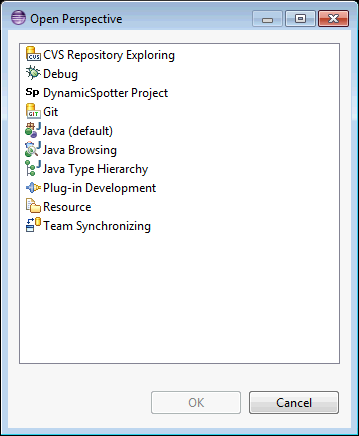
\includegraphics[width=0.4\textwidth]{figures/demo/0001-openPerspective.png}
\caption{Open \DS perspective}
\label{fig:openPerspective}
\end{figure}

\subsubsection{Creating and Configuring a \DS Project}
The \DS Eclipse-Plugin provides the notion of \DS Project. A \DS Project covers the configuration, execution and
results of \DS for a specific scenario (i.e. system under test). For our demo application scenario we first need to
create a \DS Project. Therefore, select \texttt{New \(\rightarrow\) \DS Project} in the context menu of
DynamicSpotters's Project Navigator (cf. Figure\ref{fig:contextMenu}).
In the project wizard, a name for the project and the configuration of the connection to the \DS Service are required
(cf. Figure~\ref{fig:projectWizard}).
\begin{figure}[h]
\centering
\subfigure[Context Menu
\label{fig:contextMenu}]{
	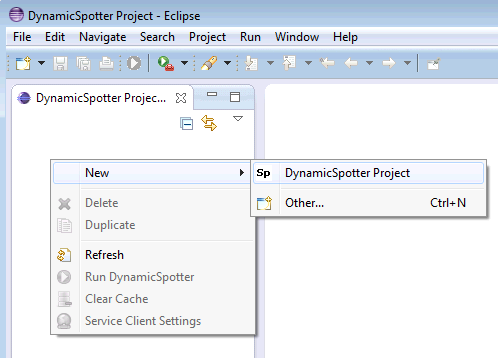
\includegraphics[width=0.47\textwidth]{figures/demo/0002-createDSProject.png}
}
\subfigure[\DS Project Wizard
\label{fig:projectWizard}]{
	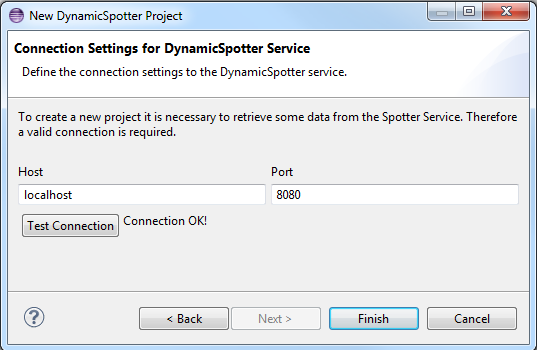
\includegraphics[width=0.47\textwidth]{figures/demo/0003-projectWizard-2.png}
}
\caption{Creating \DS Project}
\label{fig:createProject}
\end{figure}
The newly created project should now occur in the Project Navigator with a project structure as shown in
Figure~\ref{fig:projectStructure}. 
A \DS Project has two main nodes: a \texttt{Configuration} part and a \texttt{Results} part. In the
\texttt{Configuration} part, one has to specify the scenario-specific properties as well as domain specific
configuration parameters for \DS. The \texttt{\DS Config} contains global configurations and domain specific information
required for the execution of \DS on the specific system under test. The \texttt{Satellite Adapter} configurations allow
to specify the measurement environment of the scenario including configuration of instrumentation, measurement and
workload adapters.

The \texttt{Results} part provides a history of results for \DS diagnosis runs
executed for that \DS Project.

\begin{figure}[h]
\centering
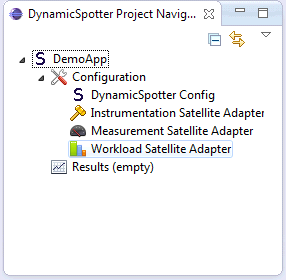
\includegraphics[width=0.4\textwidth]{figures/demo/0004-navigation.png}
\caption{Project Structure}
\label{fig:projectStructure}
\end{figure}

In the following, we explain how to configure \DS for our demo scenario. First, we edit the \texttt{\DS Config} by
opening (double-click on \texttt{\DS Config} in the Project Navigator) the \texttt{\DS Config Editor} (cf.
Figure~\ref{fig:confgiEditor}). 
\begin{figure}[h]
\centering
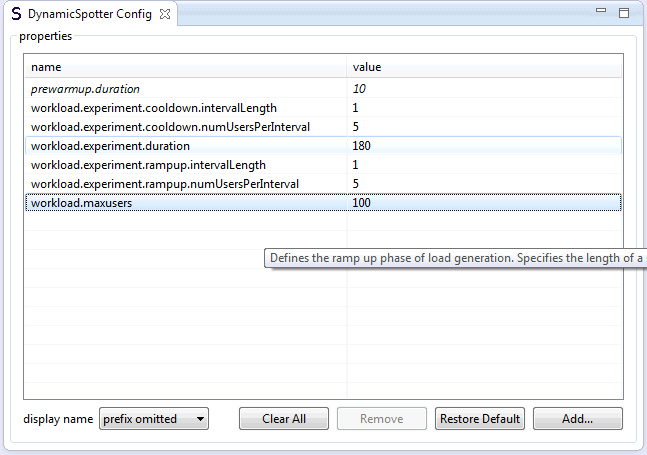
\includegraphics[width=0.8\textwidth]{figures/demo/0005-configEditor.png}
\caption{\DS Config Editor}
\label{fig:confgiEditor}
\end{figure}
We can edit the individual properties like experiment duration, maximal
expected number of users, etc. The tool tip on each property shows the description of that property. 
\DS requires six parameters specifying the workload to be mandatory configured for a certain scenario (parameters
starting with \texttt{workload.*}). Additionally to the mandatory properties, one can configure optional properties. 
Therefore, add an optional property by clicking on the \texttt{Add\ldots} button at the bottom right, and select a
parameter you would like to edit.
For our demo scenario we use a configuration as depicted in Figure~\ref{fig:confgiEditor}: We set the duration of
the initial warm-up phase (\texttt{prewarmup.duration}) of the system under test to 10 seconds. Each experiment should
be executed for 180 seconds (\texttt{workload.experiment.duration}), and for the ramp-up and cool-down behaviour of each
experiment we define a user entry rate of that 5 users per second. Furthermore, we expect a maximum number of 100
users for our demo scenario (\texttt{workload.maxusers}). 
Finally, we save that configuration.

As next step we specify the measurement environment. As you may remember, in Section~\ref{sec:demoApp} we started the
demo application with an instrumentation agent. That agent covers the functionality of two \DS Satellite Adapter types:
it is responsible for instrumenting the target application (\texttt{Instrumentation Satellite Adapter}) and in order to
retrieve the measurement data generated by the instrumentation code that agent provides an interface for a
\texttt{Measurement Satellite Adapter}. Furthermore, besides that two adapters we will need to configure a
\texttt{Workload Satellite Adapter} using the load script described in Section~\ref{sec:loadScript}.


We start with specifying the instrumentation adapter. Therefore, we need to open the editor for \texttt{Instrumentation
Satellite Adapters}. There, we add an instrumentation adapter of type
\texttt{instrumentation.satellite.adapter.default}( \texttt{Add\ldots} button on the upper part of the editor).
\begin{figure}[h]
\centering
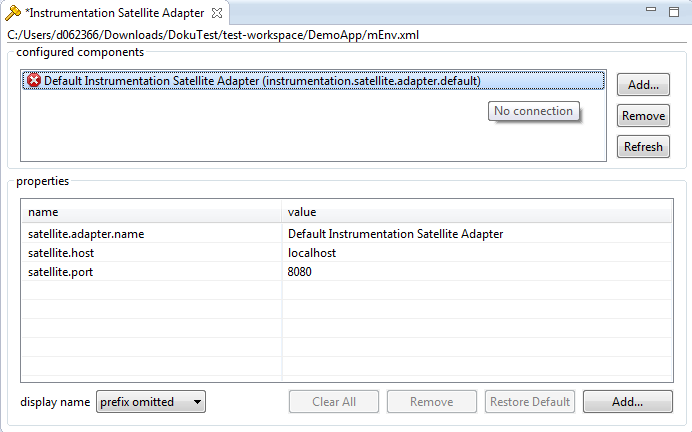
\includegraphics[width=0.8\textwidth]{figures/demo/0007-instrumentationEditor.png}
\caption{\DS Instrumentation Satellite Adapter Editor}
\label{fig:instrumentationEditor}
\end{figure}
We then see a instrumentation adapter entry in the list with a red cross (cf. Figure~\ref{fig:instrumentationEditor}).
The red cross means that no connection to the satellite could be established. As mentioned in Section~\ref{sec:demoApp}, the instrumentation agent starts per default
its REST service on port \texttt{8888}. Thus, we need to change the port in the properties view of the
instrumentation adapter (\texttt{satellite.port}) from \texttt{8080} to \texttt{8888}. This should turn the red cross to
a green check mark. Again, we need to save the configuration.
Analogously to the configuration of the instrumentation adapter we have to create a measurement adapter in the
\texttt{Measurement Satellite Adapter} editor. Thereby, we need a measurement adapter of type
\texttt{measurement.satellite.adapter.instrumentation} in order to connect to the measurement interface of the
instrumentation agent. 

Finally, we have to configure a workload adapter. Therefore, we open the \texttt{Workload Satellite Adapter Editor} and
add a satellite of the type \texttt{workload.satellite.adapter.customized} (cf. Figure~\ref{fig:workloadConfig}). This
type of workload adapter is a simple load generator which runs within the \DS process. Therefore, this adapter does not have properties like host or port and
is per default connected to \DS (green check mark). The customized workload adapter uses a Java class extending the
interface \texttt{ISimpleVUser} (cf. Section~\ref{sec:loadScript}) as a load script for a virtual user. Thus, we need to
specify the full qualified class name of that load script class (\texttt{workload.simple.userScriptClassName}) and the
path (\texttt{workload.simple.userScriptPath}) to the directory containing the Java package structure (the
\texttt{loadScript} directory of the all-in-one-drop archive).

\begin{figure}[h]
\centering
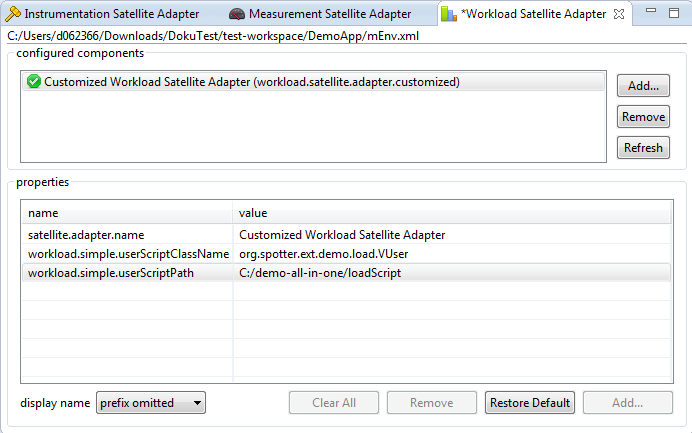
\includegraphics[width=0.8\textwidth]{figures/demo/0012-workloadConfig.png}
\caption{Configuration of the Workload Adapter}
\label{fig:workloadConfig}
\end{figure}

Having configured the global properties and specified the measurement environment, our \DS Project is ready to be
executed. Therefore select the \texttt{DemoApp} project in the \DS Project Navigator and click on the \texttt{Run}
button (or \texttt{Run DynamicSpotter} in the context menu of the Project Navigator).
In general, depending on the complexity of the scenario the execution of \DS may take hours. The execution of our demo
scenario may take up to 30 minutes. 

\subsubsection{Analyzing \DS Results}



\subsection{Executing \DS from Command Line}
\label{sec:usingCommandLine}
When using the Eclipse-Plugin to configure a \DS Project, the Eclipse-Plugin creates configuration files for \DS in the
background (which you can find in the project directory in your Eclipse workspace).
In order to execute \DS from the command line, \DS configuration files need to be passed to \DS directly instead of
executing the steps from Section~\ref{sec:usingEclipseUI}. 
First, adapt the paths in the \texttt{demo-config/spotter.conf} of the all-in-one-drop. In particular, set the paths to
the hierarchy XML, the measurement environment XML and the result directory 
When adapted use the following command to start \DS from the command line:
\begin{lstlisting}[language=sh,morekeywords={java,javaagent,port, rootDir}, frame=single]
java -jar ds-cl-runner.jar <PATH_TO_SPOTTER_CONF>
\end{lstlisting}
Thereby, the \texttt{<PATH\_TO\_SPOTTER\_CONF>} points to the \DS configuration as provided with the all-in-one-drop
(\texttt{demo-config/spotter.conf}). During execution, \DS writes the measurement and detection results to the specified
result directory.



\section{Building \DS}
\label{sec:buildingDynamicSpotter}
In order to build the \DS framework, the following tools need to be installed:
\begin{itemize}
  \item JDK (tested with JDK
  1.7)\\ \link{http://www.oracle.com/technetwork/java/javase/downloads/jdk7-downloads-1880260.html}
  \item Git client \\ \link{http://git-scm.com/downloads}
  \item Maven 3 \\ \link{http://maven.apache.org/download.cgi}
\end{itemize}

In Section~\ref{sec:links}, we provide some useful Web links including the link to the \DS framework repository. 
Use a Git client to clone the repository from the \DS GitHub repository:
\newline
\newline
\link{https://github.com/sopeco/DynamicSpotter}
\newline
\newline
The \DS framework comprises seven sub-projects:

\begin{table}[h]
\centering
\begin{tabular}{p{0.23\textwidth}p{0.7\textwidth}}
\toprule
 \textbf{Project Name} & \textbf{Description}\\
\midrule
org.spotter.parent & Maven parent project for the \DS framework\\
\midrule
org.spotter.core & Comprises the core of the \DS framework\\
\midrule
org.spotter.runner & Wraps a command line executor around \DS core\\
\midrule
org.spotter.service & Wraps a Web server around \DS core extending it with a REST service layer.\\
\midrule
org.spotter.client & The \DS client is used to conveniently consume the \DS REST service from other applications using
the org.spotter.client library.\\
\midrule
org.spotter.shared & Comprises classes and artifacts shared between \DS core, \DS runners and \DS client\\
\midrule
org.spotter.eclipse.ui & The Eclipse-Plugin provides a graphical user interface for configuring, executing \DS and
analyzing its detection results. This project uses the \DS client to communicate with the \DS REST service.\\
\bottomrule
\end{tabular}
\caption{\DS Project Structure}
\label{tab:projects}
\end{table}

In order to build dynamic spotter use the command line and switch to the \texttt{org.spotter.parent} directory. There,
execute the following Maven build command:
\begin{lstlisting}[language=sh,morekeywords={java,javaagent,port, rootDir}, frame=single]
mvn clean install
\end{lstlisting}
If executed successfully, Maven creates in the \texttt{target} directories of the individual sub-projects the
corresponding JARs. The executable JAR for the \DS Service is located in the \texttt{org.spotter.service/target}
directory. 

The Eclipse Plugin JAR is located in the \texttt{org.spotter.eclipse.ui/target} directory.

\section{Writing Extensions for \DS}
\label{sec:extensions}
As mentioned in Section~\ref{sec:architecture}, \DS provides four different types of extensions which are required to
run \DS. These types are explained in Section~\ref{sec:architecture}. A collection of some extensions for \DS is
available under the following GitHub repository:
\newline
\newline
\link{https://github.com/sopeco/DynamicSpotter-Extensions}
\newline
\newline
In this section, we explain how to write different types of extensions for \DS.

\subsection{General Structure of a \DS Extension}
\label{sec:extensionsGeneralStructure}
\DS extensions can be either bundled in separate JARs or in aggregated JARs each containing several extensions.
A single extension at least comprises a Java class providing meta-information about the extension (with typical suffix
\texttt{\_\_\_Extension}), a Java class representing the actual extension artifact, and an entry in a text file
declaring the extension. The extension class has to implement at least three methods (cf.
Listing~\ref{lst:iExtension}). 
\lstinputlisting[language=Java, frame=single,
caption=Methods to be
implemented by an
Extension Class,commentstyle=\color{mygreen},keywordstyle=\color{blue},stringstyle=\color{mymauve},tabsize=3,
label=lst:iExtension]{code/IExtension.txt} The \texttt{getName} method specifies the name of the extensions, the \texttt{getConfigParameters} method allows to define a set of extension-specific configuration parameters, and the
\texttt{createExtensionsArtifacts} method creates the actual extension artifact. The extension artifact needs to
pass an instance of the extension class as the extension provider to the super constructor (cf.
Listing~\ref{lst:ExtensionArtifact}).
\lstinputlisting[language=Java, frame=single,
caption=A constructor of
an Extension Artifact,commentstyle=\color{mygreen},keywordstyle=\color{blue},stringstyle=\color{mymauve},tabsize=3,
label=lst:ExtensionArtifact]{code/ExtensionArtifact.txt}
Finally, we have to declare the extension in the \texttt{extensions.info} file. The \texttt{extensions.info} file
contains per extension a line with the full qualified name of the corresponding extension (provider) class (cf.
Listing~\ref{lst:extensionsInfo}).
\lstinputlisting[language=Java, frame=single,
caption=Declaring an extension in the \texttt{extensions.info}
file,commentstyle=\color{mygreen},keywordstyle=\color{blue},stringstyle=\color{mymauve},tabsize=3, label=lst:extensionsInfo]{code/extensions.info}
The \texttt{extensions.info} file needs to be located in a directory called \texttt{plugins}.
Assuming that we bundle each extension in a separate JAR, despite for additional dependencies the JAR structure would
look like as follows:
\dirtree{%
 .1 /.
 .2 org.
 .3 \ldots.
 .4 MyExtension.class.
 .4 MyExtensionArtifact.class.
 .2 plugins.
 .3 extensions.info.
}

In the following, we describe for each extension type what needs to implemented to provide an extension for the
corresponding type.

\subsection{Writing an Instrumentation Extension}
As explained in Section~\ref{sec:extensionsGeneralStructure}, for an extension we need an \emph{extension artifact
class} implementing the functionality of the extension type and an \emph{extension class} providing meta information on
the extension. Except for the class to inherit, the extension class has the same structure for the extension types
\emph{Instrumentation, Measurement and Load Generation} (cf. Listing~\ref{lst:instExtension}). 
\lstinputlisting[language=Java, frame=single,
caption=Extension class
for an instrumentation
extension,commentstyle=\color{mygreen},keywordstyle=\color{blue},stringstyle=\color{mymauve},tabsize=3,
label=lst:instExtension]{code/instExtension.txt}
An instrumentation extension needs to inherit the class \texttt{AbstractInstrumentationExtension}. \texttt{getName}
returns the unique name of the extension. In the \texttt{initializeConfigurationParameters} method we can provide a
textual description of the extension as well as a set of extension-specific configuration parameters. The
\texttt{isRemoteExtension} method indicates whether the corresponding extension is an adapter to a remote satellite. If
that is the case, \DS later uses the \texttt{testConnection} method to check whether a connection to the remote
satellite can be established. Finally, the method \texttt{createExtensionArtifact} creates a new instance of the actual
instrumentation extension artifact (here: \texttt{MyInstExtensionArtifact}). In this example the class
\texttt{MyInstExtensionArtifact} implements the actual instrumentation adapter, and as such has to inherit the class
\texttt{AbstractInstrumentationAdapter} (cf. Listing~\ref{lst:instExtensionArtifact}).
\lstinputlisting[language=Java, frame=single,
caption=Extension Artifact class
for an instrumentation
extension,commentstyle=\color{mygreen},keywordstyle=\color{blue},stringstyle=\color{mymauve},tabsize=3,
label=lst:instExtensionArtifact]{code/instExtensionArtifact.txt}
An instrumentation extension artifact has to implement three methods: \texttt{initialize, instrument} and
\texttt{uninstrument}. The \texttt{initialize} method takes care of conducting initialization tasks required before the
specific instrumentation tool can be used. The \texttt{instrument} method triggers the instrumentation, realizing the
instrumentation instructions wrapped by the instrumentation description. Finally, the \texttt{uninstrument} method
reverts the instrumentation. Depending on the tool used for instrumentation the implementation of this instrumentation
adapter may look completely different. For instance, if we are using our own instrumentation tool (Adaptable
Instrumentation and Monitoring (AIM)), the adapter just passes the instrumentation description to the remote
AIM instrumentation engine to realize the instrumentation. An instrumentation extension for Kieker or DiSL would require
to translate the instrumentation description into Kieker- or DiSL-specific instrumentation instructions. Furthermore, if
the instrumentation tool does not support dynamically adaptable instrumentation, the instrumentation extension would
need to take care of restarting the target application to enable adaptation of the instrumentation state.
Regardless of which instrumentation tool is used behind an instrumentation extension, \DS only assumes that after
calling the \texttt{instrument} method, the target application is instrumented accordingly. Analogously for the
\texttt{uninstrument} method.


\subsection{Writing a Measurement Extension}
A measurement extension class has to inherit the class \texttt{AbstractMeasurmentExtension}. Apart from that, the
extension class of a measurement extension has the same structure as shown in Listing~\ref{lst:instExtension}. A
measurement extension artifact has to inherit the class \texttt{AbstractMeasurmentAdapter} exhibiting a structure as
depicted in Listing~\ref{lst:measExtensionArtifact}.
\lstinputlisting[language=Java, frame=single,
caption=Extension Artifact class
for a measurement
extension,commentstyle=\color{mygreen},keywordstyle=\color{blue},stringstyle=\color{mymauve},tabsize=3,
label=lst:measExtensionArtifact]{code/measExtensionArtifact.txt}
Analogously to the instrumentation adapter, a measurement adapter can be initialized. The \texttt{enableMonitoring} and
\texttt{disableMonitoring} activate data gathering on the target system. The methods \texttt{getMeasurementData} and
\texttt{pipeToOutputStream} allow to retrieve the data measured since the last activation of monitoring. While
\texttt{getMeasurementData} is a blocking call, \texttt{pipeToOutputStream} allows to take advantage of data pipelining.
Finally, \texttt{getCurrentTime} returns the current timestamp of the monitoring tool. This timestamp is required to
align the timestamps of all records which may come from distributed system nodes.
Analogously to instrumentation extensions, a measurement extension serves as an adapter. For instance, if we want
to use Kieker as monitoring tool, the corresponding measurement extension has to take care of translating Kieker
monitoring records into the DynamicSpotter-specific representation of measurement data. In this way, we enable the usage
of diverse tools via the adapters while keeping a consistent data representation within \DS.

\subsection{Writing a Load Generation Extension}
A load generation extension class has to inherit the class \texttt{AbstractWorkloadExtension}. Apart from that, the
extension class of a measurement extension has the same structure as shown in Listing~\ref{lst:instExtension}.
A load generation extension artifact has to inherit the class \texttt{AbstractWorkloadAdapter} yielding a class
structure as depicted in Listing~\ref{lst:wlExtensionArtifact}.
\lstinputlisting[language=Java, frame=single,
caption=Extension Artifact class
for a load generation
extension,commentstyle=\color{mygreen},keywordstyle=\color{blue},stringstyle=\color{mymauve},tabsize=3,
label=lst:wlExtensionArtifact]{code/wlExtensionArtifact.txt}
Same as for the instrumentation and measurement adapters, a workload adapter provides a method for initialization tasks.
By calling the \texttt{startLoad} method, \DS tells a workload adapter to start generating load \emph{asynchronously}. 
The three \texttt{wait\_\_\_} methods block until the corresponding experiment phase has been reached.
In our extensions repository (cf. Section~\ref{sec:links}), we provide load generation adapters for Apache JMeter,
HP~LoadRunner, and a simple custom workload generator used in the Demo example in Section~\ref{sec:demoApp}.


\subsection{Writing a Detection Heuristic}
In the \DS framework the detection heuristics for individual performance problems are managed as extensions, as well.
The extension class of a detection heuristic extension has to extend the class \texttt{AbstractDetectionExtension}. 
The three methods which need to be implemented we already know from the general structure shown in
Listing~\ref{lst:iExtension}. The class implementing the actual detection logic has to extend the
\texttt{AbstractDetectionController} class. This inheritance requires the detection class to implement four methods as
shown in Listing~\ref{lst:detectionHeuristic}.
\lstinputlisting[language=Java, frame=single,
caption=Detection controller class
for a detection heuristic
extension,commentstyle=\color{mygreen},keywordstyle=\color{blue},stringstyle=\color{mymauve},tabsize=3,
label=lst:detectionHeuristic]{code/detectionHeuristic.txt}
The \texttt{loadProperties} method is called by \DS directly after the instantiation of the detection class. This method
can be used to load heuristic-specific properties as defined in the \texttt{getConfigParameters} method of the extension
class (cf. Listing~\ref{lst:iExtension}). The detection process of an individual heuristic comprises two phases: an
experiment execution phase and an data analysis phase. While the former is triggered by the \texttt{executeExperiments}
method, the \texttt{analyze} method is responsible for analysing the measured data and return a detection result.
For the experiment phase, a detection heuristic has to specify a problem-specific instrumentation of the target
application by providing an instrumentation description. (Note: this instrumentation description should be system
independent in order to be reused in other systems as well.) Using the instrumentation description the detection
heuristic can tell the \DS to execute a series of experiments (cf. \texttt{executeDefaultExperimentSeries}) using the
corresponding instrumentation, measurement and load generation adapters. \texttt{defaultExperimentSeries} means that a
set of \texttt{n} experiments is executed, whereby the load is increased from one experiment to the next between a load
of 1 user and the specified maximum number of users. When the experimentation phase has finished, \DS calls the
\texttt{analyze} method passing the measured data as input to that method. It is now up to the analyze method to apply
certain detection rules in order to provide a detection result. A detection result has to state whether the
corresponding analyzed performance problem has been detected or not.
Finally, the \texttt{getNumOfExperiments} method is used by \DS to estimate the duration of the experiments. In this
method, the developer of a detection heuristic has to provide the number of experiments executed for that heuristic.

\section{Useful Links}
\label{sec:links}
\begin{table}[h]
\centering
\begin{tabular}{p{0.45\textwidth}p{0.45\textwidth}}
\toprule
 \textbf{Link} & \textbf{Description}\\
\midrule
\midrule
\multicolumn{2}{c}{\mbox{\textbf{Code Repositories}}}\\
\midrule
\small{\link{https://github.com/sopeco/DynamicSpotter}} & \DS framework
repository\\
\midrule
\small{\link{https://github.com/sopeco/DynamicSpotter-Extensions}}
& Extensions repository for \DS\\
\midrule
\small{\link{https://github.com/sopeco/LPE-Common}} & Repository containing
utility libraries for performance measurements, data analysis, load generation, etc.\\
\midrule
\multicolumn{2}{c}{\mbox{\textbf{Documentation}}}\\
\midrule
\small{\link{http://sopeco.github.io/DynamicSpotter}}
& Documentation on \DS\\
\midrule
\small{\textcolor[rgb]{0.0,0.0,1.0}{\href{http://i43vm-saas.ipd.uka.de:8082/artifacts/javadoc/DynamicSpotter/v1}{http://i43vm-saas.ipd.uka.de:8082/artifacts/
javadoc/DynamicSpotter/v1}}} & JavaDoc for the \DS framework\\
\midrule
\multicolumn{2}{c}{\mbox{\textbf{Build Infrastructure}}}\\
\midrule
\small{\link{http://i43vm-saas.ipd.uka.de:8082/jenkins/}}
& Jenkins build server for \DS related projects. Contains statistics on Findbugs, Checkstyle, Unit-Tests, Test
coverage etc.\\
\bottomrule
\end{tabular}
\caption{Useful Links}
\label{tab:usefulLinks}
\end{table}

\bibliographystyle{IEEEtranSA}
\bibliography{doc}

\end{document}
